%!TEX root = ../template.tex

\section{Experimental Design}
%
Data were collected at Istituto Italiano di Tecnologia (IIT), Genoa, Italy. The experimental
set-up encompasses the following different sensor modules: 
$j)$ a wearable suit for the motion tracking,
$jj)$ two standard force platforms to acquire the ground reaction wrenches, 
$jjj)$ the force/torque sensors of the robot arms. 
%
%%%%%%%%%%%%%%%%%%%%%%%%%%%%%%%%%%%%%%%%%%%%%%%%%%%%%%%%%%%%%%%%%%%%%%%%%%%%%%%%%%%%%%%%%%%%%%%%
\subsection{Human configuration}
Ten healthy adult subjects (7 female, 3 male) have been recruited in the experimental 
session, height (\unit{166,6\pm4,5}{\centi\meter}) and 
mass (\unit{61,14\pm5,76}{\kilo\gram}).
Each subject was provided of a written informative consent before starting the experiment. Kinematics
  data were acquired by using a full-body wearable lycra suit provided by Xsens Technologies.  
The wearable suit is composed of 17 wired trackers, (i.e., inertial sensor units-IMUs including an
 accelerometer, a gyroscope and a magnometer). The suit has signal transmitters that send
  measurements to the acquisition unit through a wireless receiver which collects data at a
   frequency of \unit{240}{\hertz}. The human subject performed the required
    task standing with the
   feet on two standard force platforms AMTI OR6 mounted on the ground, while interacting 
   with the robot.
	  Each platform acquired a wrench sample at a frequency of
	   \unit{1}{\kilo\hertz} by using AMTI acquisition units. 
%
\begin{figure}
  \centering
    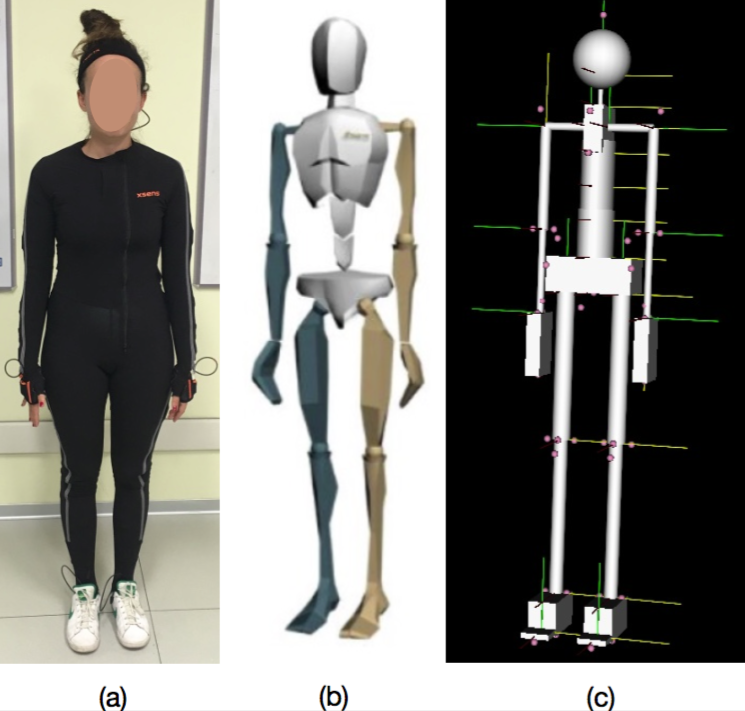
\includegraphics[width=0.9\columnwidth]{figs/humanModels}
  \caption{(a) Subject with the motion capture suit. (b) The Xsens MVN model. (c) Model reconstructed in OpenSim by using virtual markers from Xsens acquisition.}
 \label{fig:human_models}
\end{figure}
%
%%%%%%%%%%%%%%%%%%%%%%%%%%%%%%%%%%%%%%%%%%%%%%%%%%%%%%%%%%%%%%%%%%%%%%%%%%%%%%%%%%%%%%%%%%%%%%%%
\subsection{Robot configuration}
Experiments were conducted on the iCub \cite{Metta2010}, a full-body humanoid
robot (Fig. \ref{fig:iCub_couple}a) with 53-DoFs: 6 in the head, 16 in each arm, 3 in the
 torso and 6 in each leg. The iCub is endowed with whole-body distributed force/torque sensors,
  accelerometers, gyroscopes and tactile sensors. Specifically, the limbs are equipped with six
   force/torque sensors placed in the upper arms, in the upper legs and in the ankles 
   (Fig. \ref{fig:iCub_couple}b). Internal joint torques and external wrenches are estimated
    through an online whole-body estimation algorithm \cite{Nori2015icub}. Measurements for the
    wrenches exchanged between the robot and the human are obtained thanks to it.  Robot data
	 were collected at a frequency of \unit{100}{\hertz}.
%
\begin{figure}
  \centering
    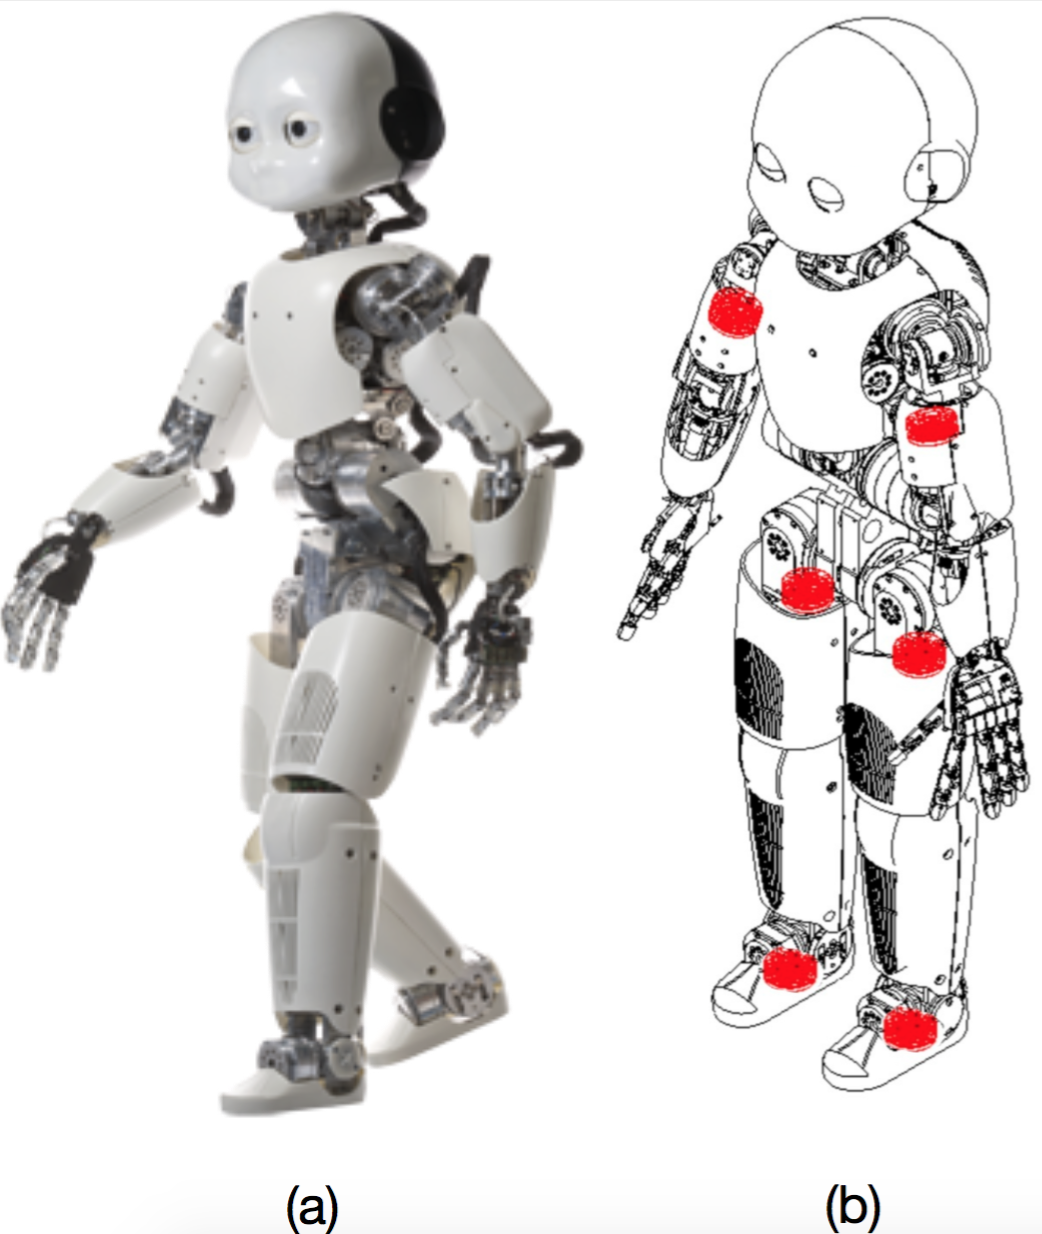
\includegraphics[width=0.75\columnwidth]{figs/iCub_couple}
  \caption{(a) The humanoid iCub. (b) Model of the iCub with the force/torque 
  sensors embedded in the limbs structure.}
  \label{fig:iCub_couple}
\end{figure}
%
%%%%%%%%%%%%%%%%%%%%%%%%%%%%%%%%%%%%%%%%%%%%%%%%%%%%%%%%%%%%%%%%%%%%%%%%%%%%%%%%%%%%%%%%%%%%%%%%
\subsection{Procedure protocol}
Each subject was asked to wear the suit (Fig. \ref{fig:human_models}a) and to stand on the 
two force plates by positioning each foot per platform. The robot 
  was located in front of the subject facing him at a known distance from the human foot
   location (as shown in Fig. \ref{fig:interaction_lateral&top}a). The mutual feet position was
    fixed for all the trials (Fig. \ref{fig:interaction_lateral&top}b).  
	The interaction implied that the human grasped and pushed down both robot arms 
	(Fig. \ref{fig:interaction_lateral&top}a) for those tasks that required the interaction.
	The subject performed:
	\begin{itemize}
		\item a bowing task ($BT$) without (Fig. \ref{fig:sequenceTask}a) and with
		 (Fig. \ref{fig:sequenceTask}b) the robot interaction;
		\item a squat task ($ST$) without (Fig. \ref{fig:sequenceTask}c) and with
		 (Fig. \ref{fig:sequenceTask}d) the robot.
		\end{itemize} 
All subjects had to perform five repetitions of the block composed of the above-mentioned
 tasks. In each block the order of tasks execution was randomized in order to make each 
trial as independent as possible among the blocks.
%
\begin{figure}[ht]
  \centering
    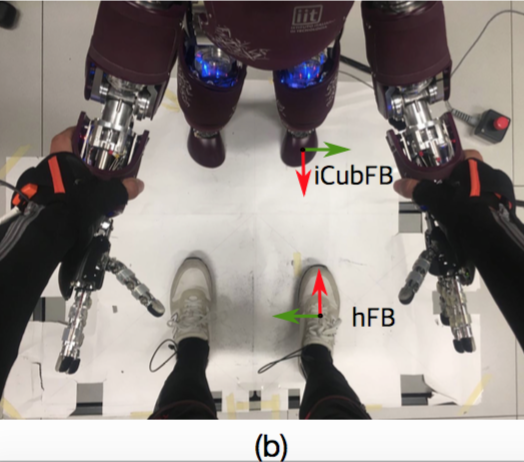
\includegraphics[width=6cm]{figs/interaction_lateralAndTop}
          \caption{(a)  Subject grasps and pushes down the robot arms.  The figure shows the
		  reference frames for the force/torque sensor of the robot (iCubFT), the robot fixed
		   base (iCubFB), the force plate (FP), the human fixed base (hFB), the human foot and
		    hand (hFOOT, hHAND) respectively. (b) Top view for the fixed feet position layout.}
			\label{fig:interaction_lateral&top}
\end{figure}
%
% \begin{figure}[h]
%   \centering
%    \begin{subfigure}[b]{0.5\columnwidth}
%       \includegraphics[width=\textwidth]{figs/interactionFrames.pdf}
%           \caption{}
%           \label{fig:figs_interactionFrames}
%   \end{subfigure}
%    \begin{subfigure}[b]{0.6\columnwidth}
%     \includegraphics[width=\textwidth]{figs/fixedTopView.pdf}
% 	\caption{}
%         \label{fig:fixedPositionTospView}
%    \end{subfigure}
%           \caption{(a)  Subject grasps and pushes down the robot arms.  The figure shows the
% 		  reference frames for the force/torque sensor of the robot (iCubFT), the robot fixed
% 		   base (iCubFB), the force plate (FP), the human fixed base (hFB), the human foot and
% 		    hand (hFOOT, hHAND) respectively. (b) Top view for the fixed feet position layout.}
% \end{figure}
%
\begin{figure*}[!ht]
  \centering
    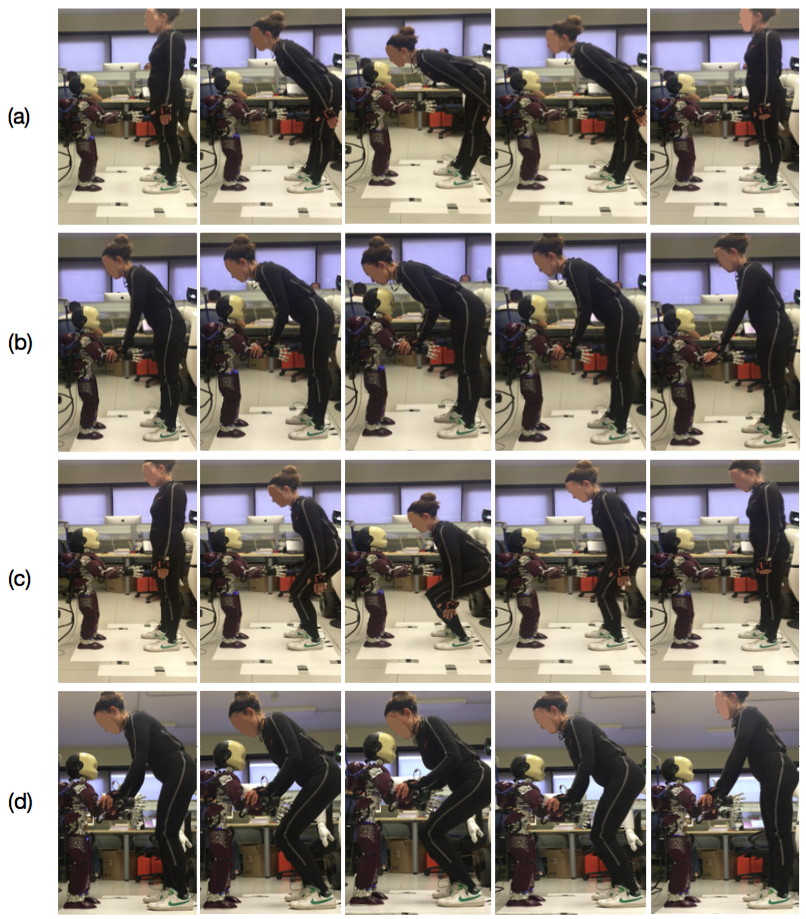
\includegraphics[width=0.75\textwidth]{figs/sequenceTask}
		  \caption{Subject performing: a $BT$ without (a) and with (b) the iCub,
		  a $ST$ without (c) and with (d) the iCub.}
			\label{fig:sequenceTask}
\end{figure*}
%
 % \begin{figure*}[h!]
 % 	 \centering
 % 	\begin{subfigure}[b]{0.7\textwidth}
 % 		\includegraphics[width=\textwidth]{figs/h_bowing.pdf}
 % 		\caption{}
 % 		\label{fig:h_bowing}
 % 	 \end{subfigure}
 % 	\begin{subfigure}[b]{0.7\textwidth}
 % 		\includegraphics[width=\textwidth]{figs/hri_bowing.pdf}
 % 		\caption{}
 % 		\label{fig:hri_bowing}
 % 	 \end{subfigure}
 % 	\begin{subfigure}[b]{0.7\textwidth}                                                                 \includegraphics[width=\textwidth]{figs/h_squat.pdf}
 % 		  	\caption{}
 % 		  	\label{fig:h_squat}
 % 	 \end{subfigure}
 %  	\begin{subfigure}[b]{0.7\textwidth}                                                                 \includegraphics[width=\textwidth]{figs/hri_squat.pdf}
 % 		  	\caption{}
 % 		  	\label{fig:hri_squat}
 %  	 \end{subfigure}
 %     \caption{Subject performing: a $BT$ without (a) and with (b) the iCub,
 % 	 a $ST$ without (c) and with (d) the iCub.}
 % \end{figure*}
%
%%%%%%%%%%%%%%%%%%%%%%%%%%%%%%%%%%%%%%%%%%%%%%%%%%%%%%%%%%%%%%%%%%%%%%%%%%%%%%%%%%%%%%%%%%%%%%%%
\subsection{Data processing}
Since the acquisition sampling rate was different among the sources, data are linearly
 interpolated in order to guarantee the synchronization. An overview of the framework is
  summarised in Fig. \ref{fig:figs_schemeAlgorithm}. Data coming from the force plates and from
   the robot (${\bm f^x}$) are considered as acquired from a particular class of net external
    wrench sensors. Linear acceleration $\bm a$ and angular velocity $\bm \omega$ for each
	 link are acquired by Xsens inertial sensors.
Xsens data are used as input for the OpenSim \cite{Delp2007} IK (Inverse Kinematics)
 toolbox that allowed to retrieve the joint angles $\bm q$ by matching 
 the marker positions of the OpenSim model (Fig. \ref{fig:human_models}c) and the virtual
 ones coming from Xsens data.
 Joint velocities $\bm {\dot q}$ and accelerations $\bm {\ddot q}$  are
    computed by using a weighted sum of windows of elements, with a third-order polynomial
	 Savitzky-Golay filtering. Also joint accelerations are considered as acquired from
	  a class of DoF acceleration sensors. In general, by considering as inputs data acquired
	   from all above-mentioned sensors and the state $(\bm q,\bm {\dot q})$, the MAP
	    estimator provides the estimation of $\bm d$ given $\bm y$.
%
% \begin{figure}[h]
%   \centering
%    \begin{subfigure}[b]{1\columnwidth}
%     \includegraphics[width=\textwidth] {figs/ExpSetUp.pdf}
%         \caption{}
%         \label{fig:devicesScheme}
% \end{subfigure}
%  \begin{subfigure}[b]{0.9\columnwidth}
%     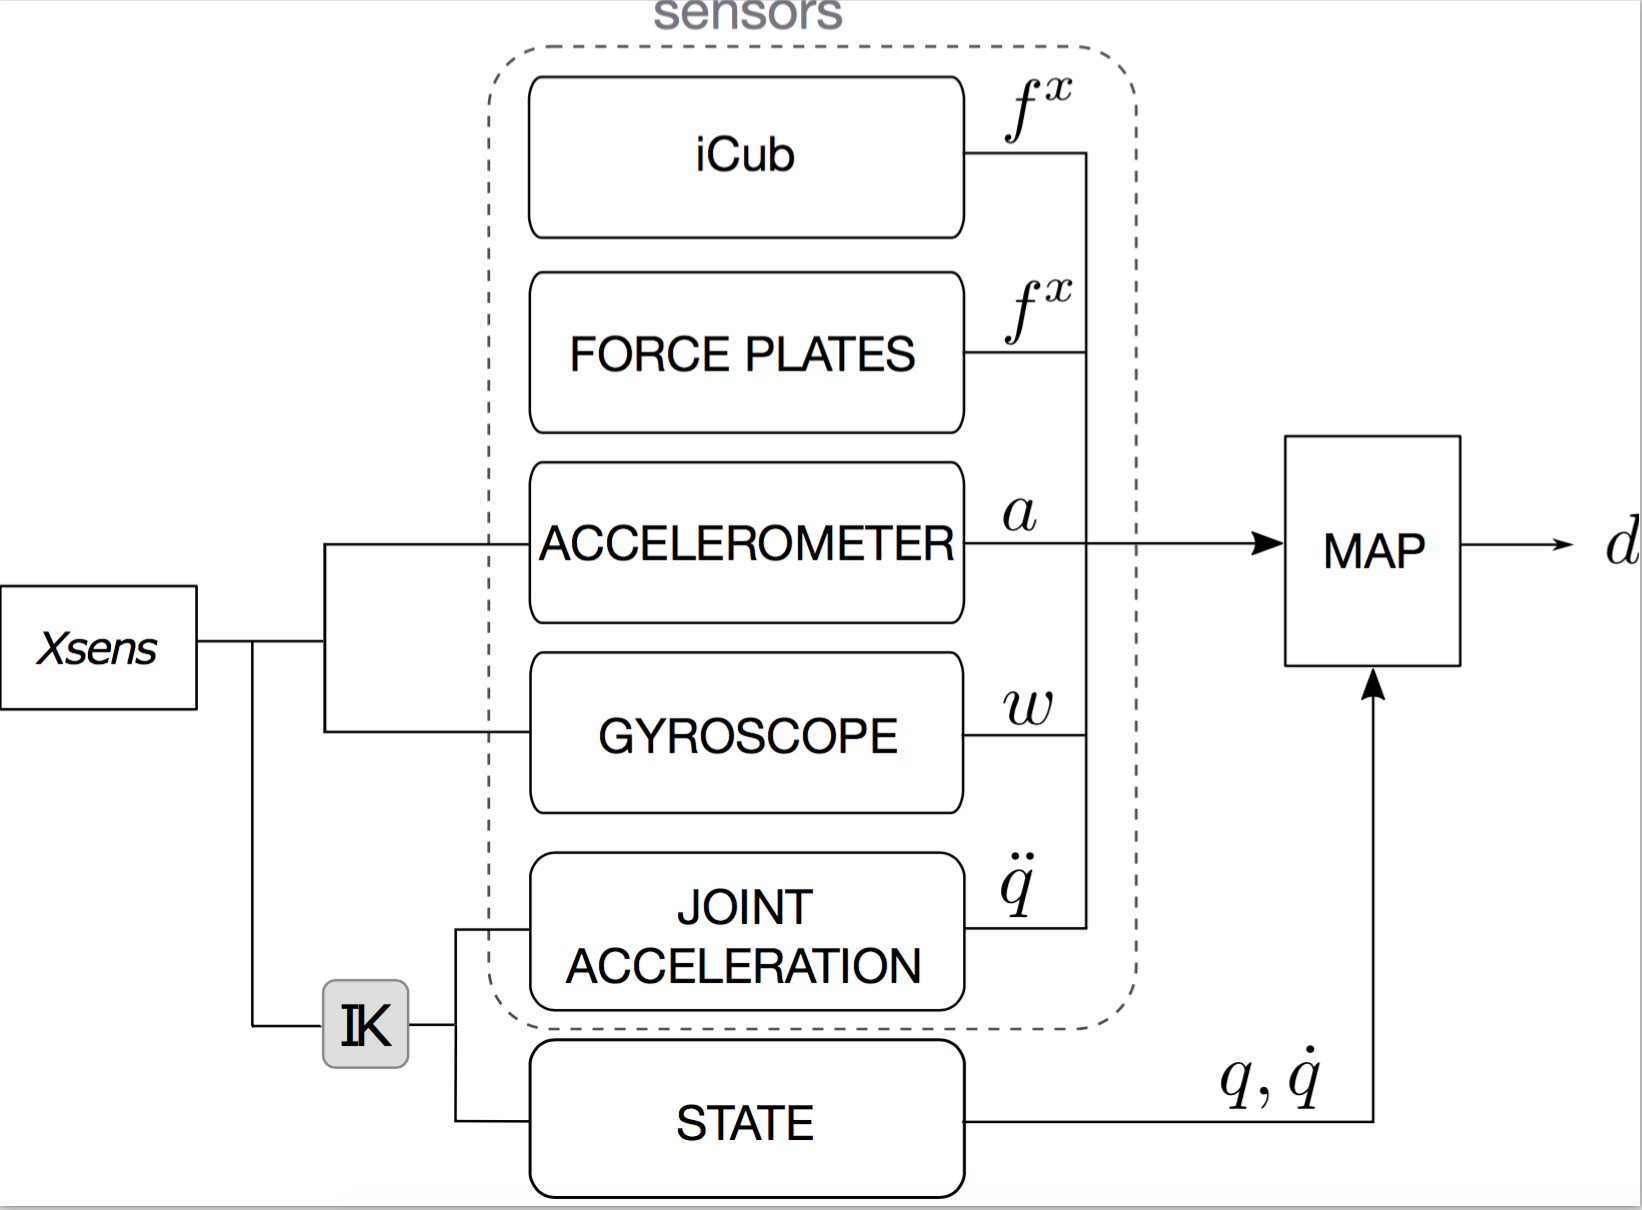
\includegraphics[width=\textwidth]{figs/schemeAlgorithm.pdf}
%         \caption{}
%         \label{fig:algorithmScheme}
% \end{subfigure}
%   \caption{(a) (b)xxx}
%   \label{fig:overview}
% \end{figure}

% \begin{figure}
% 	\centering
% 	  \def\svgwidth{0.9\columnwidth}
% 	  \import{figs/}{drawing.pdf_tex}
% \end{figure}
%
\begin{figure}
  \centering
    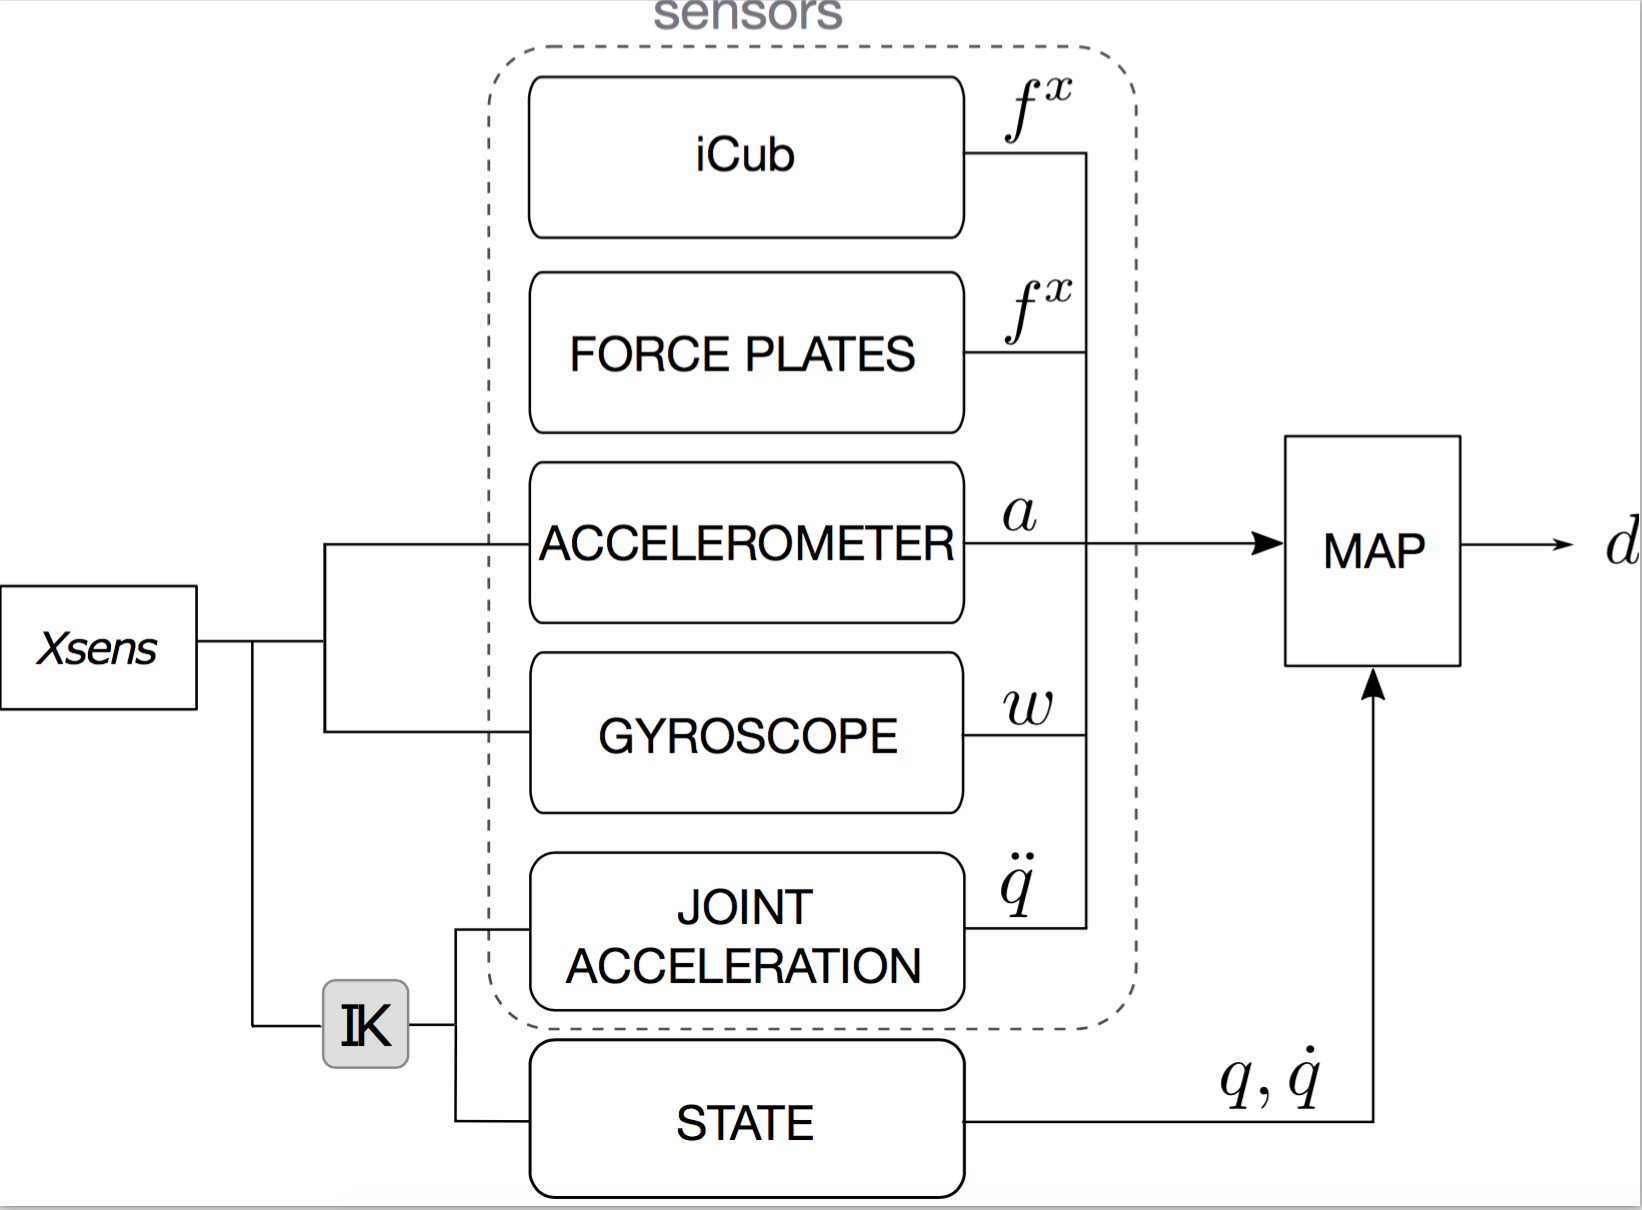
\includegraphics[width=1\columnwidth]{figs/schemeAlgorithm}
  \caption{Overview of the MAP estimation algorithm.} 
  \label{fig:figs_schemeAlgorithm}
\end{figure}